\section{References}

\begin{frame}
  \frametitle{Books}
  \begin{columns}
    \column{0.85\textwidth}
    \small
    \begin{itemize}
    \item {\bf Mastering Embedded Linux, 3rd Edition}
      \footnote{\tiny
\url{https://www.packtpub.com/product/mastering-embedded-linux-programming-third-edition/9781789530384}}\\
      By Chris Simmonds, Packt Publishing, May 2021\\
      An up-to-date resource covering most aspects of embedded Linux
      development.
    \item {\bf The Linux Programming Interface}
      \footnote{\tiny \url{https://man7.org/tlpi/}}\\
      Michael Kerrisk (maintainer of Linux manual pages), 2010, No Starch Press\\
      A gold mine about Linux system programming\\
    \item {\bf Embedded Linux System Design and Development}
      \footnote{\tiny \url{https://www.amazon.com/Embedded-Linux-System-Design-Development/dp/0849340586}}\\
      P. Raghavan, A. Lad, S. Neelakandan, Auerbach, Dec. 2005.\\
      Very good coverage of the POSIX programming API (still up
      to date).
    \end{itemize}
    \normalsize
    \column{0.15\textwidth}
    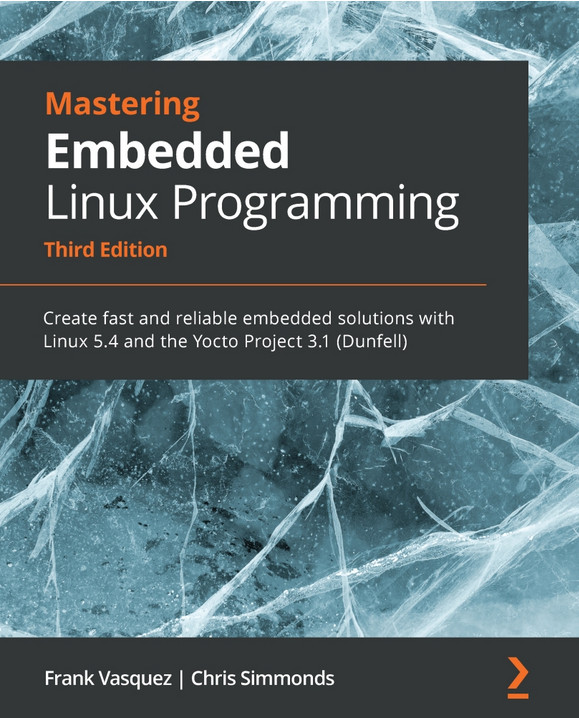
\includegraphics[height=0.25\textheight]{slides/sysdev-references/book-mastering-embedded-linux3.jpg}\\
    \vspace{0.5cm}
    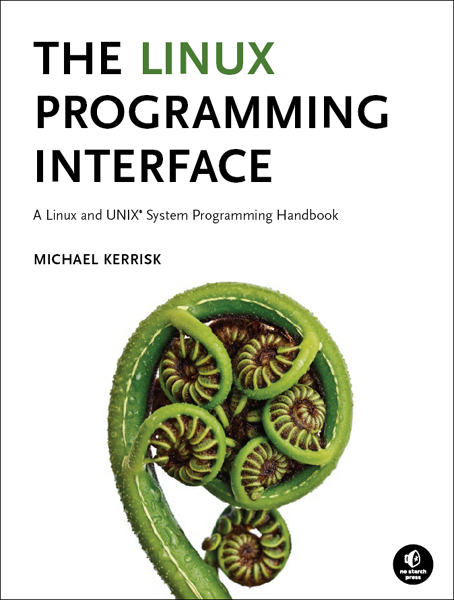
\includegraphics[height=0.25\textheight]{common/linux-programming-interface.png}\\
    \vspace{0.5cm}
    \includegraphics[height=0.25\textheight]{slides/sysdev-references/book-embedded-linux-sysdev.jpg}\\
  \end{columns}
\end{frame}

\begin{frame}
  \frametitle{Web sites}
  \begin{itemize}
  \item {\bf ELinux.org}, \url{https://elinux.org}, a Wiki entirely
    dedicated to embedded Linux. Lots of topics covered: real-time,
    filesystems, multimedia, tools, hardware platforms,
    etc. Interesting to explore to discover new things.
  \item {\bf LWN}, \url{https://lwn.net}, very interesting news site
    about Linux in general, and specifically about the kernel. Weekly
    edition, available for free after one week for non-paying
    visitors.
  \item {\bf Linux Gizmos}, \url{https://linuxgizmos.com}, a news site
    about embedded Linux, mainly oriented on hardware platforms
    related news.
  \end{itemize}
\end{frame}

\begin{frame}
  \frametitle{International conferences (1)}
  \begin{columns}
  \column{0.7\textwidth}
    \begin{itemize}
    \item Embedded Linux Conference:
  \begin{itemize}
  \item \url{https://embeddedlinuxconference.com/}
  \item Organized by the Linux Foundation
  \item Once per year, alternating North America/Europe
  \item Very interesting kernel and user space topics for embedded
        systems developers. Many kernel and embedded project maintainers are present.
  \item Presentation slides and videos freely available on
    \url{https://elinux.org/ELC_Presentations} 
  \end{itemize}

    \item Linux Plumbers
  \begin{itemize}
  \item \url{https://linuxplumbersconf.org}
  \item About the low-level plumbing of Linux: kernel, audio, power
    management, device management, multimedia, etc.
  \item Not really a conventional conference with formal
    presentations, but rather a place where contributors on each topic
    meet, share their progress and make plans for work ahead.
  \end{itemize}

    \end{itemize}
  \column{0.3\textwidth}
     \includegraphics[width=\textwidth]{common/elc-logo.png}\\
     \vspace{1cm}
     \includegraphics[width=\textwidth]{common/lpc-logo.jpg}\\
  \end{columns}
\end{frame}

\begin{frame}
  \frametitle{International conferences (2)}
  \begin{itemize}
  \item FOSDEM: \url{https://fosdem.org} (Brussels, February)\\
    For developers. Presentations about system development.
  \item Live Embedded Event: \url{https://live-embedded-event.com/}\\
	A new free live event about embedded topics. Co-organized by
        Bootlin!
  \item Currently, most conferences are available on-line. They
        are much more affordable and often free.
  \end{itemize}
\end{frame}
